\documentclass[a4paper,12pt]{ujarticle}
\usepackage{listings,jlisting}
\usepackage[top=15truemm,bottom=15truemm,left=20truemm,right=20truemm]{geometry}
\usepackage[dvips]{graphicx}
\usepackage{siunitx}
\begin{document}
\title{マイクロコンピュータ 後期期末レポート}
\author{電気情報工学科2年 \\ E1533 西総一朗}
\date{2017年2月10日提出}
\maketitle
\begin{itemize}
 \item \large 光が流れるプログラム(片道バージョン)
 \item 光が流れるプログラム(往復バージョン)
 \item パルスモータ1-2相励磁プログラム
 \item 電子サイコロのプログラム
 \item タイマ割り込み制御プログラム
\end{itemize}
\clearpage
\tableofcontents
\clearpage
 \section{リスト5-5(光が流れるプログラム(片道バージョン))}
  \subsection{プログラム概要}
  8個あるLEDの1個を右端や左端から順次点灯することによって、光が流れるように見えるプログラム。
  \subsection{フローチャート}
  このプログラムのフローチャートを図\ref{fig:flow_5-5}に示す。
  \begin{figure}[htbp]
   \begin{center}
     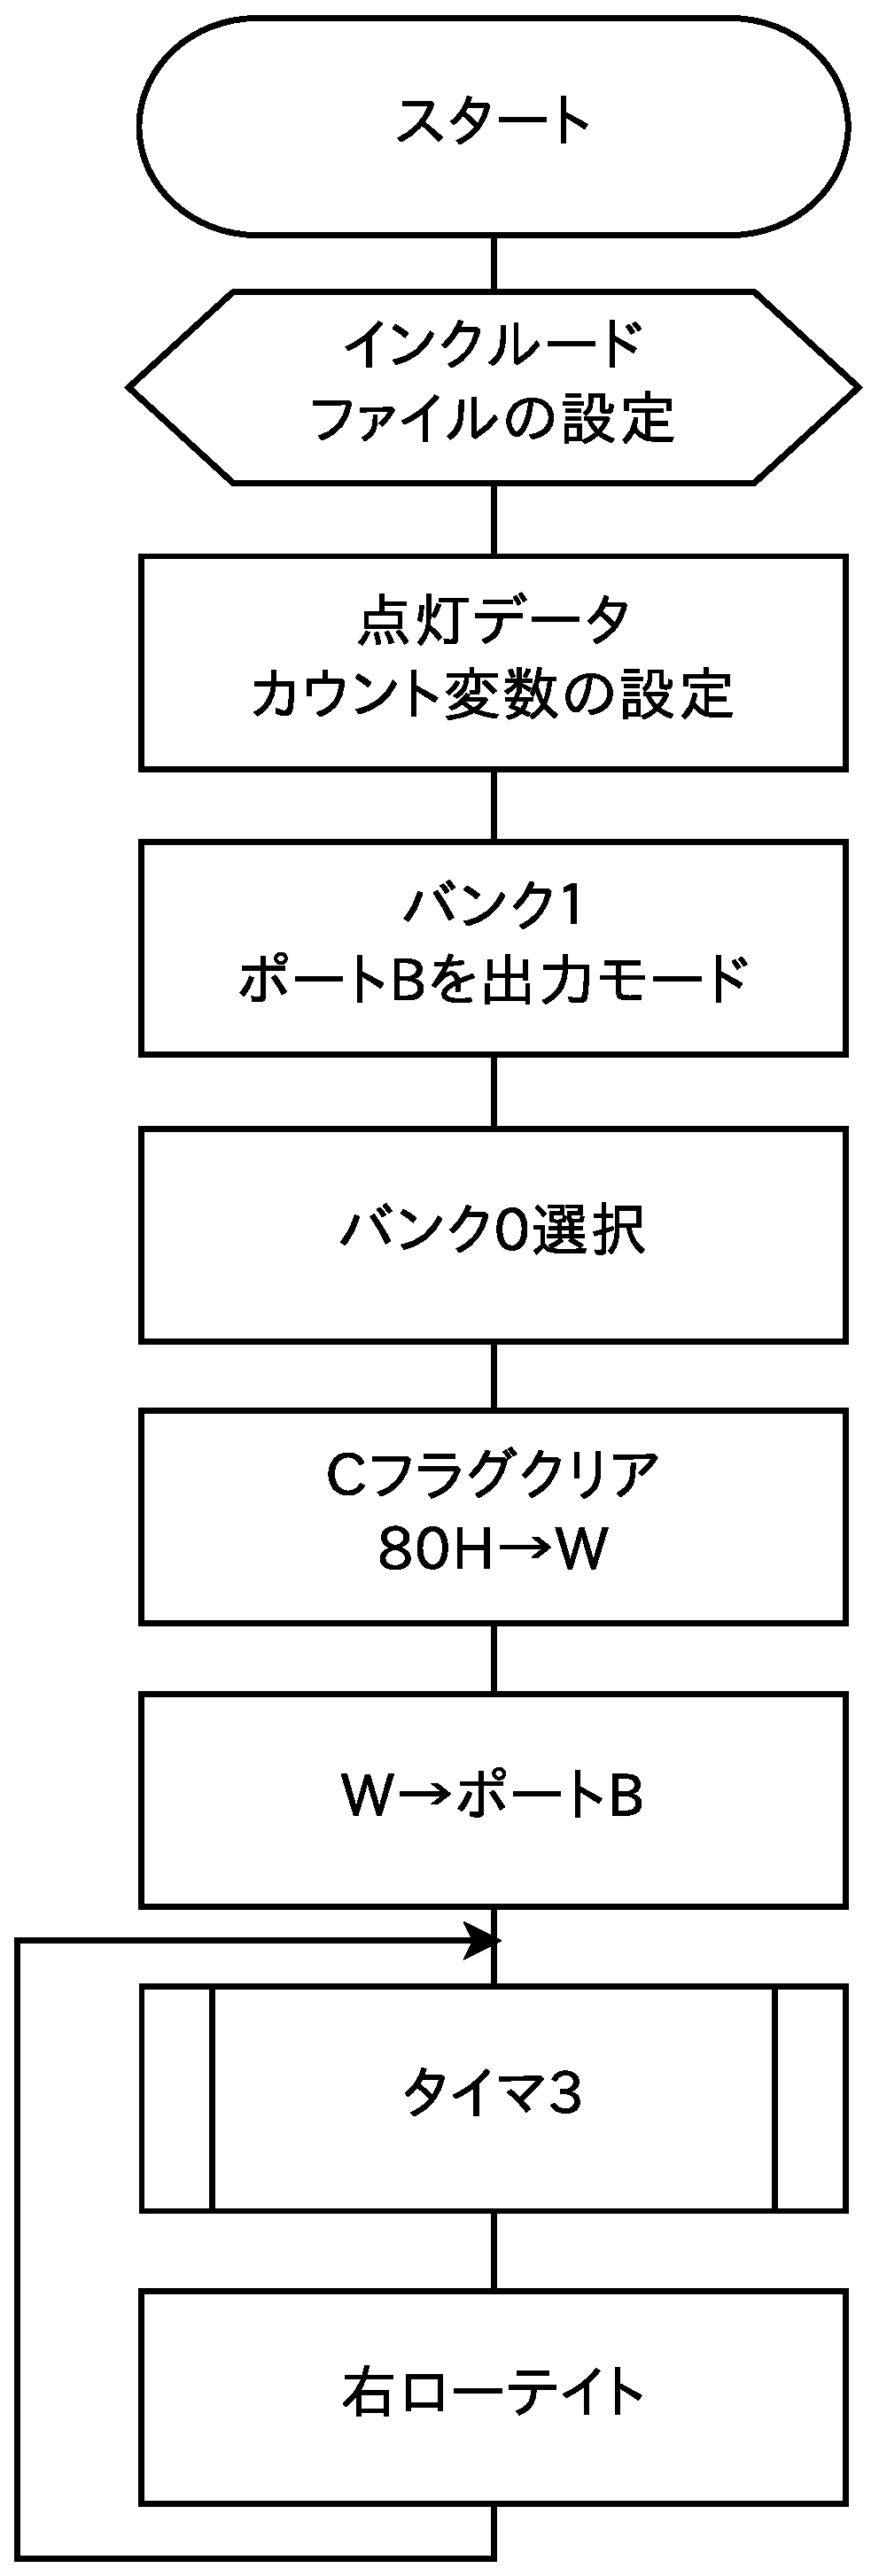
\includegraphics[height=185mm]{Diagram5-5.eps}
   \end{center}
   \caption{光が流れるプログラム ( 片道バージョン )のフローチャート}
   \label{fig:flow_5-5}
  \end{figure}
   \clearpage
  \subsection{ソースコード}
   \begin{lstinputlisting}[basicstyle=\ttfamily\footnotesize, frame=single,numbers=left]
    {../5-5/5-5.asm}
   \end{lstinputlisting}
   \clearpage
  \subsection{実行結果・考察}
   \begin{figure}[htbp]
    \begin{center}
     \begin{tabular}{cc}
      {80}$_{16}$ = 10000000$_2$ \\
      ●○○○○○○○ & □\\
      {40}$_{16}$ = 01000000$_2$ \\
      ○●○○○○○○ & □\\
      {20}$_{16}$ = 00100000$_2$ \\
      ○○●○○○○○ & □\\
      {10}$_{16}$ = 00010000$_2$ \\
      ○○○●○○○○ & □\\
      {08}$_{16}$  = 00001000$_2$ \\
      ○○○○●○○○ & □\\
      {04}$_{16}$  = 00000100$_2$ \\
      ○○○○○●○○ & □\\
      {02}$_{16}$  = 00000010$_2$ \\
      ○○○○○○●○ & □\\
      {01}$_{16}$  = 00000001$_2$ \\
      ○○○○○○○● & □\\
      {00}$_{16}$  = 00000000$_2$ \\
      ○○○○○○○○ & ■\\
     \end{tabular}\\
     ●:LED点灯 ○:LED消灯,■:Cフラグ1 □:Cフラグ0
    \end{center}
   \caption{光が流れるプログラム ( 片道バージョン )の実行結果}
   \label{fig:out_5-5}
   \end{figure}
   図\ref{fig:out_5-5}ように、0.5秒毎に光る場所が右に動き、右端に到達するとすべてのLEDが消えるタイミングがある。
   ローテイト(RRF)命令は1ビットずつ右にシフトさせるもので、16進数において1ビット右にシフトさせることは2で割ることになる。
   RRF命令はCフラグを経由してデータを回転するので端に到達したら一時的に全部が消える瞬間がある。
   \\

   このプログラムのタイマについて考察してみる。

   PICのクロック周波数は$10\si{\mega\hertz}$なので、1クロックあたりは
    \[
     \frac{1}{10\si{\mega\hertz}} = \SI{0.1}{\mu\second}
    \]
    4クロックで1サイクルなので、1サイクルあたりは
    \[
     \SI{0.1}{\mu\second} \times 4 = \SI{0.4}{\mu\second}
    \]
     \begin{figure}[h]
      \begin{center}
       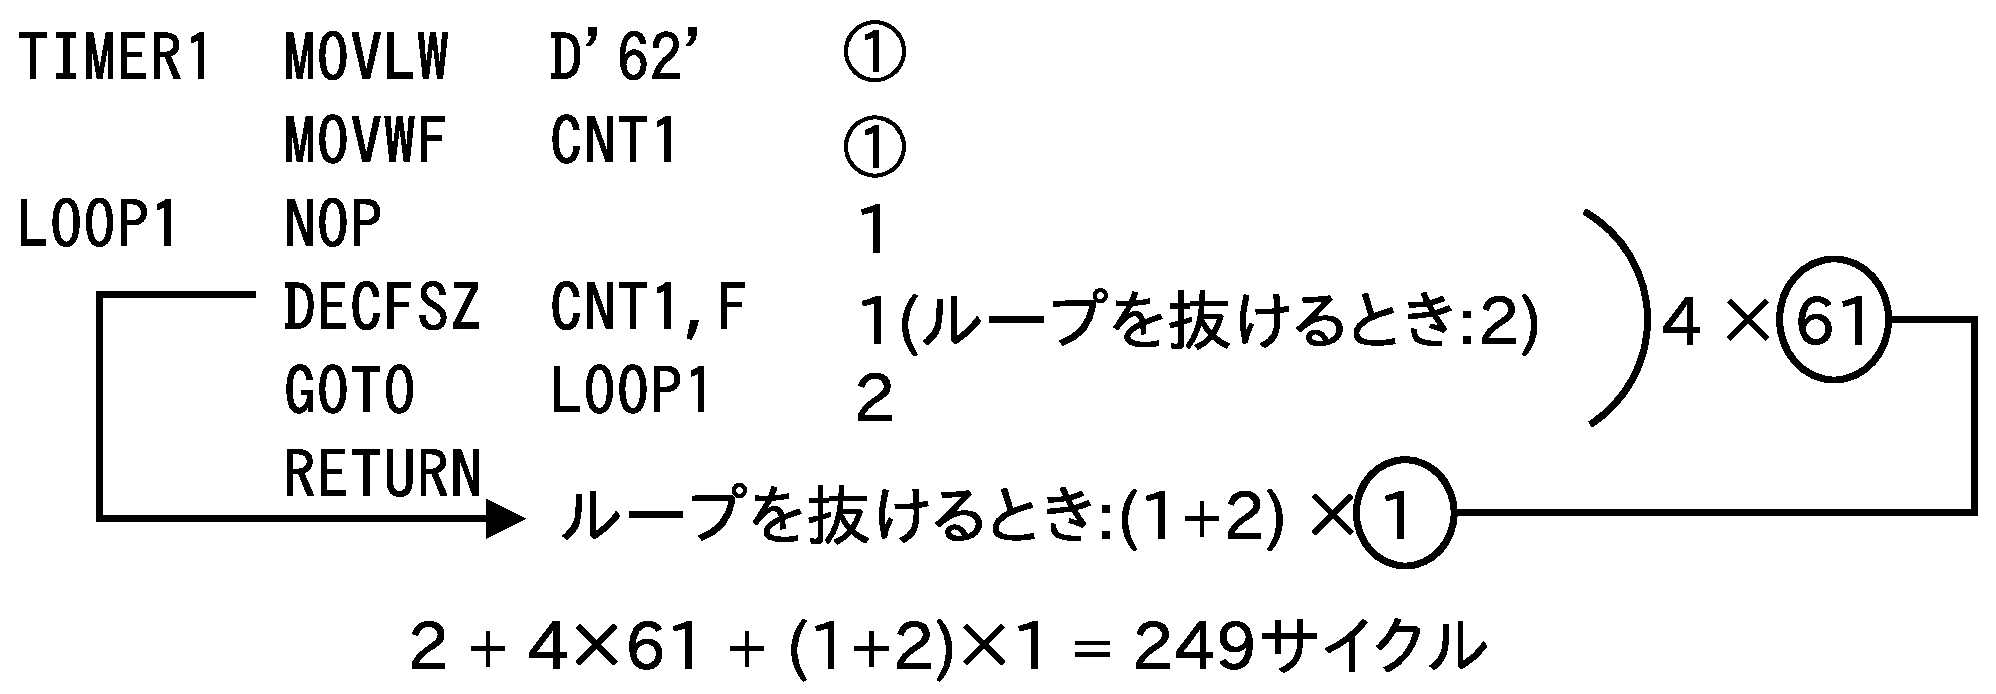
\includegraphics[width=130mm]{Diagram5.eps}
      \end{center}
      \caption{サイクル数の考え方}
      \label{fig:sicle}
     \end{figure}
     TIMER1のサイクル数は図\ref{fig:sicle}より、249サイクルだとわかり、
     \[
      \SI{0.4}{\mu\second} \times 249 = \SI{99.6}{\mu\second} \approx \SI{0.1}{\milli\second}
     \]
     TIMER1では$\SI{0.1}{\milli\second}$消費される。\\
     このTIMER1をTIMER2では100回、TIMER2では50回呼び出しているので、
     \[
      \SI{0.1}{\milli\second} \times 100 \times 50 = \SI{50}{\milli\second} = \SI{0.5}{\second}
     \]
    よって合計で$\SI{0.5}{\second}$のタイマールーチンであることがわかる。

     ローテイト(RRF)命令を0.5秒のタイマルーチン毎に呼び出すことで、0.5秒毎に光が動いているように見える。
     \\

     次に光の移動方向について考察してみる。

     このプログラムにおいて、光の移動方向を決めているのは
      \begin{lstlisting}[basicstyle=\ttfamily\footnotesize, frame=single]
 9行目     LEDD    EQU     80H     ;LEDの点灯データの設定

24行目     RRF     PORTB,1         ;ポートBを1ビット右にローテイト
      \end{lstlisting}

      この2つなので、次のように変更すれば左方向に移動するようになる。
      \begin{lstlisting}[basicstyle=\ttfamily\footnotesize, frame=single]
 9行目     LEDD    EQU     01H     ;LEDの点灯データの設定

24行目     RLF     PORTB,1         ;ポートBを1ビット右にローテイト
      \end{lstlisting}

      RLF命令もRRF命令と同様に、Cフラグを経由してデータを回転するので、端に到達したら一時的に全部が消える。

      LEDの移動時間$S$を調整するにはTIMER1の0.1ミリ秒を基準にして、
      \begin{eqnarray*}
       S = \SI{0.1}{\milli\second} \times {\rm TIMER2 \times TIMER3} \\
       {\rm TIMER2 \le 255},\ 
       {\rm TIMER3 \le 255}
      \end{eqnarray*}
      TIMER2とTIMER3でループ回数を決める。
 \clearpage
 \section{リスト5-6(光が流れるプログラム(往復バージョン))}
  \subsection{プログラム概要}
  8個LEDの1個を左端や右端から順次点灯していき、端に到達したら逆方向に点灯させることでLEDの点灯が、往復して流れるように見えるプログラム。
  \subsection{フローチャート}
  \begin{figure}[htbp]
   \begin{center}
    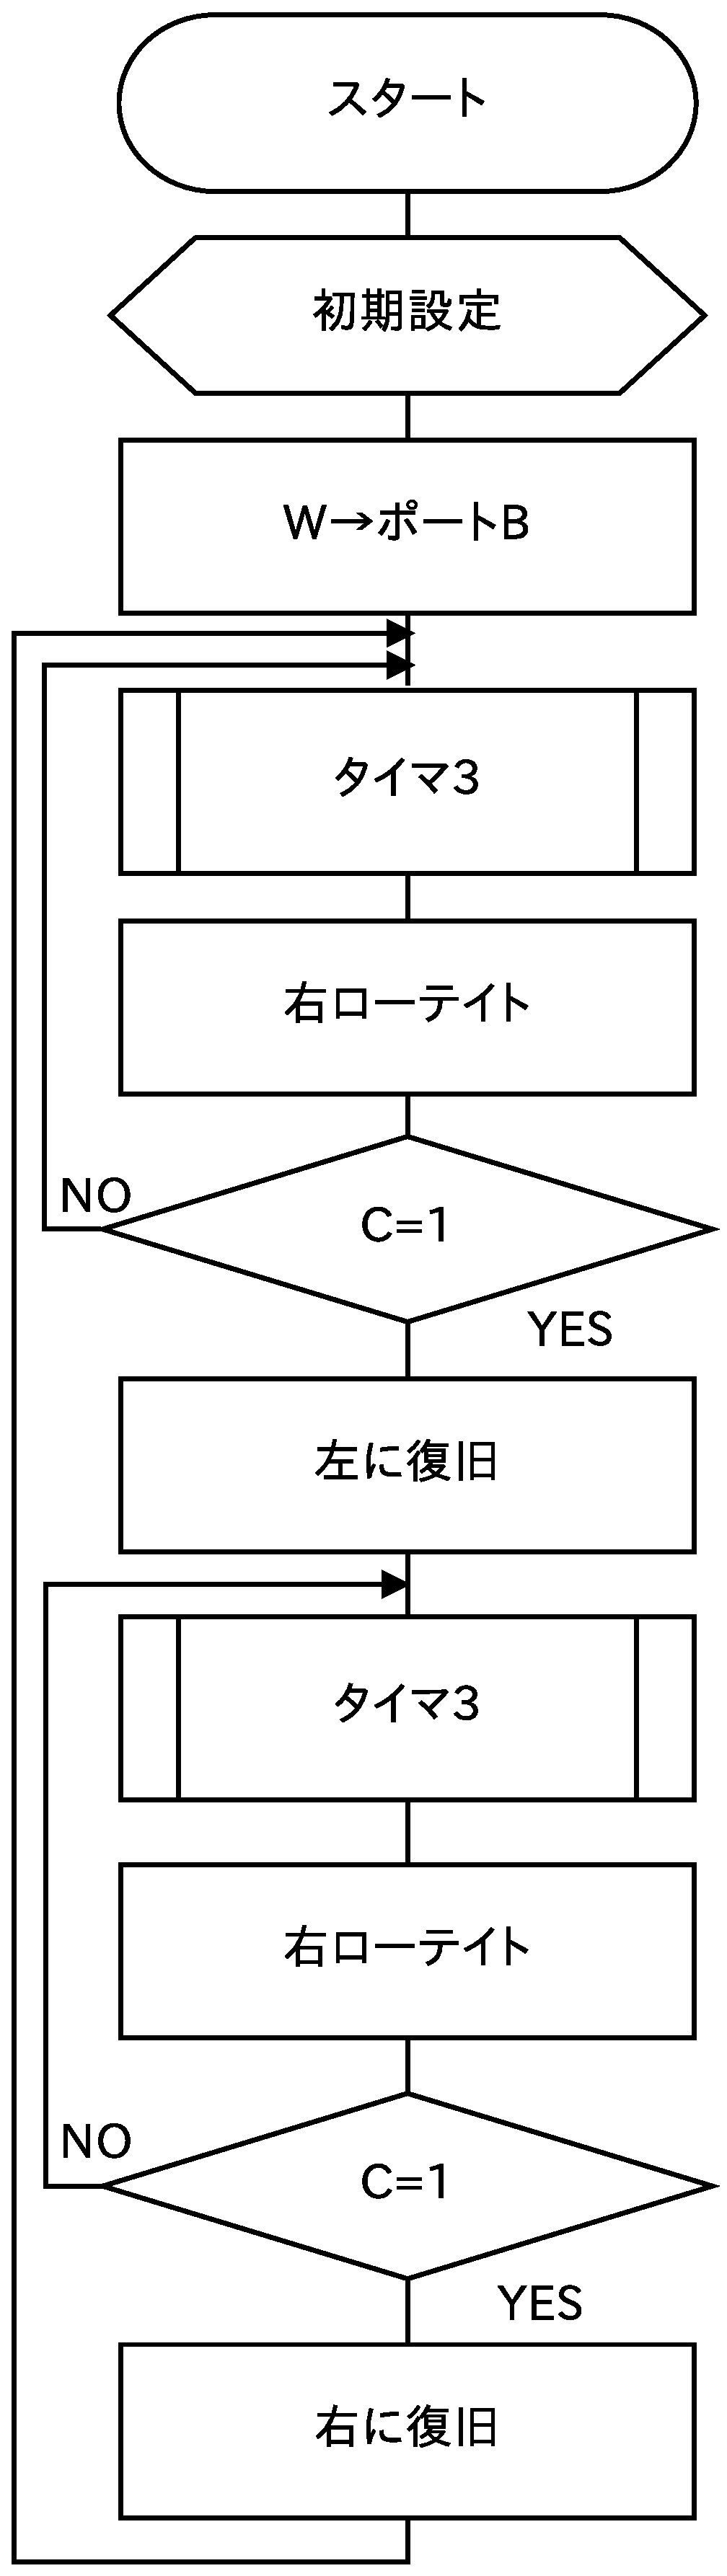
\includegraphics[height=180mm]{Diagram5-6.eps}
   \end{center}
   \caption{光が流れるプログラム ( 往復バージョン )のフローチャート}
   \label{fig}
  \end{figure}
  \clearpage
  \subsection{ソースコード}
   \begin{lstinputlisting}[basicstyle=\ttfamily\footnotesize, frame=single,numbers=left]
   {../5-6/5-6.asm}
   \end{lstinputlisting}
   \subsection{実行結果・考察}
   \begin{figure}[htbp]
    \begin{center}
     \begin{tabular}{c|c}
      {80}$_{16}$ = 10000000$_2$ & {01}$_{16}$  = 00000001$_2$ \\
      ●○○○○○○○            & ○○○○○○○● \\
      {40}$_{16}$ = 01000000$_2$ & {02}$_{16}$  = 00000010$_2$ \\
      ○●○○○○○○            & ○○○○○○●○ \\
      {20}$_{16}$ = 00100000$_2$ & {04}$_{16}$  = 00000100$_2$ \\
      ○○●○○○○○            & ○○○○○●○○ \\
      {10}$_{16}$ = 00010000$_2$ & {08}$_{16}$  = 00001000$_2$ \\
      ○○○●○○○○            & ○○○○●○○○ \\
      {08}$_{16}$  = 00001000$_2$ & {10}$_{16}$ = 00010000$_2$ \\
      ○○○○●○○○            & ○○○●○○○○ \\
      {04}$_{16}$  = 00000100$_2$ & {20}$_{16}$ = 00100000$_2$ \\
      ○○○○○●○○            & ○○●○○○○○ \\
      {02}$_{16}$  = 00000010$_2$ & {40}$_{16}$ = 01000000$_2$ \\
      ○○○○○○●○            & ○●○○○○○○ \\
      {01}$_{16}$  = 00000001$_2$ & {80}$_{16}$ = 10000000$_2$ \\
      ○○○○○○○●            & ●○○○○○○○ \\
     \end{tabular}\\
     ●:LED点灯 ○:LED消灯
     \caption{光が流れるプログラム ( 往復バージョン )の実行結果。左の列のあと右の列が実行される。}
     \label{fig:out_5-6}
    \end{center}
   \end{figure}
   図\ref{fig:out_5-6}のように左端から、0.2秒毎に光るところが右に動いていき右端になったら、移動方向を左にして移動する。
   \\
   ローテイト命令(RRF,RLF)は、Cフラグを含めてシフトするので、光が右端(0ビット目)または左端(7ビット目)に移動したことをCフラグで判定している。
   Cフラグが1の場合はオーバーフローかアンダーフローしているので、図\ref{fig:under}のように過分ローテイトの復旧(2ビット復旧)することで、なめらかに移動するように見える。

   \begin{figure}[htbp]
    \begin{center}
      \begin{tabular}{ccl}
      76543210 & C  & \\
      {01}$_{16}$ = 00000001$_2$ \\
      ○○○○○○○● & □ & 0ビット目点灯 \\
      {00}$_{16}$ = 00000000$_2$ \\
      ○○○○○○○○ & ■ & Cフラグにアンダーフロー \\
      {02}$_{16}$ = 00000010$_2$ \\
      ○○○○○○●○ & □ & 過分ローテート復旧(RLF $\times$ 2) \\
      \end{tabular}\\
     ●:LED点灯 ○:LED消灯,■:Cフラグ1 □:Cフラグ0
     \caption{過分ローテート復旧の例}
     \label{fig:under}
    \end{center}
   \end{figure}
   光の移動方向については、過分ローテートの復旧を行っているため、LEDの点灯データを変えるだけで、移動方向を変えられる。\\
   \\
   これを
   \begin{lstlisting}[basicstyle=\ttfamily\footnotesize, frame=single]
9行目    LEDD     EQU     80H    ;左端から右方向にスタート
   \end{lstlisting}
   次のように変更すれば、スタート時の移動方向を反対にできる。
   \begin{lstlisting}[basicstyle=\ttfamily\footnotesize, frame=single]
9行目    LEDD     EQU     01H    ;右端から左方向にスタート
   \end{lstlisting}

   次に過分ローテイトの復旧がない場合について考えてみる。
    \begin{figure}[htbp]
     \begin{center}
      \begin{tabular}{ccl}
       76543210 & C  & \\
       {02}$_{16}$ = 00000010$_2$ \\
       ○○○○○○●○ & □ & 1ビット目点灯 \\
       {01}$_{16}$ = 00000001$_2$ \\
       ○○○○○○○● & □ & 0ビット目点灯 \\
       {00}$_{16}$ = 00000000$_2$ \\
       ○○○○○○○○ & ■ & Cフラグにアンダーフロー \\
       {01}$_{16}$ = 00000001$_2$ \\
       ○○○○○○○● & □ & 0ビット目点灯 \\
       {02}$_{16}$ = 00000010$_2$ \\
       ○○○○○○●○ & □ & 1ビット目点灯 \\
      \end{tabular}\\
      ●:LED点灯 ○:LED消灯,■:Cフラグ1 □:Cフラグ0
      \caption{過分ローテート復旧がない場合}
      \label{fig:under}
     \end{center}
    \end{figure}
  過分ローテイトの復旧がないと、すべてのLEDが点灯しない瞬間が生じる。
  \subsection{練習問題5.10}
  \clearpage
\end{document}